\begin{textblock}{\mycolwidth}(\leftpos,2.5)
\LHead{Introduction} \\
\large
Various routing models each considering some aspects of finding ``best''
solutions:
\begin{itemize}
  \item Shortest Path Problem: Finding a shortest path also yields an efficient path regarding energy consumption.
  \item Shortest Weight-Constrained Path Problem: Optimize more than one target function, e.g.\ time and energy-consumption.
  \item Time-Dependent and Multi-Modal Routing: Finding shortest paths depending on the time, caused for example by including public transportation.
  \item Energy-Optimal Routing: Considering energy constraints for electric vehicles.
  \item Stochastic Routing: Minimizing expected costs, maybe given certain conditional probabilities.
  \item Rerouting: After finding an efficient path and turning to a different direction (or gaining additional information),
  quickly find an alternate efficient route.
\end{itemize}
Each model comes with its own set of algorithms,
our aim is to find a model unifying some aspects while still
allowing for most algorithms known for the shortest path problem.
\end{textblock}

\begin{textblock}{\mycolwidth}(\leftpos,8.25)
\LHead{Prototype} \\
The Technische Universit\"at M\"unchen (TUM) developed a prototypic routing service,
which is further developed at the University of L\"ubeck,
available at \url{www.isp.uni-luebeck.de/greennav}. It is used
to evaluate different routing algorithms. You can see a range prediction
of an electric vehicle.\\[1em]
\resizebox{5\TPHorizModule}{!}{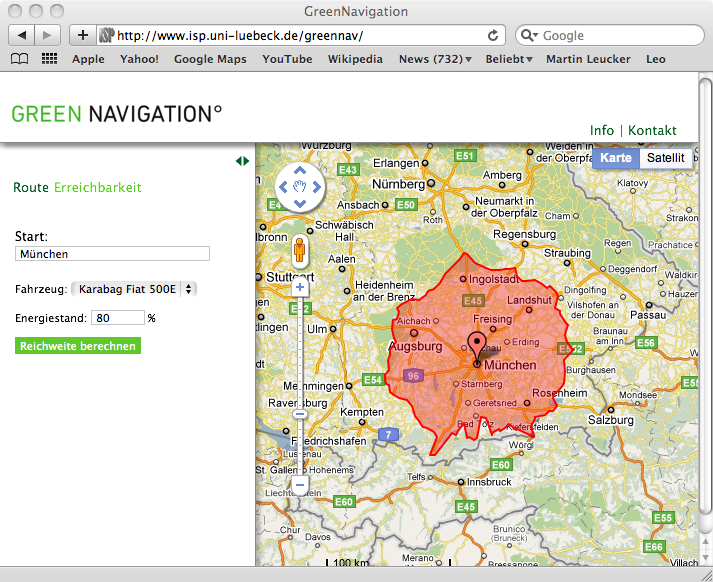
\includegraphics{greennav.png}}
\end{textblock}

\begin{textblock}{\mycolwidth}(\leftpos,14.75)
\LHead{Definition: State-Based Routing}
\begin{itemize}
  \item $G = (V, E)$ is a graph,
  \item $S$ is a set of states preordered by $\leq_S$,
  \item $\mathcal S:\ V \to \mathcal P(S)$ describes possible states at each vertex,
  \item $\mathbb W$ is a set of \emph{monotone} ($x_1 \leq_S x_2 \to f(x_1) \leq_S f(x_2)$)
  and \emph{extensive} ($x \leq_S f(x)$) weights $S \leadsto S$,
  \item $\mathcal W':\ E \to \mathbb W$ is a weighting,
\end{itemize}
such that
\begin{itemize}
  \item $\mathcal W'(x, y)$ is a weight $\mathcal S(x) \to \mathcal S(y)$, and
  \item the \emph{extension} of $\mathcal W'$ again is $\mathcal W:\ \text{walks} \to \mathbb W$ given by
  \[\mathcal W(\gamma) = \mathcal W'(v_0, v_1) \circ \ldots \circ \mathcal W'(v_{k-1}, v_k)\]
  for all walks $\gamma = (v_0, \ldots, v_k), k \geq 0$ (identity for $k = 0$).
\end{itemize}
\vspace{0.5em}
Objective:
\begin{itemize}
  \item Given $x, y \in V$ and initial state $s \in \mathcal S(x)$,
  find at least one corresponding path
  for each minimal element in $\min(\mathcal W(\text{walks from}\ x\ \text{to}\ y)(s))$
  (except for equivalence), where
  \[\min(S) := \{s \in S\ |\ \neg\exists s' \in S:\ s' < s\}.\]
\end{itemize}
\end{textblock}
